\documentclass{article}
\usepackage[utf8]{inputenc}
\usepackage{amsmath}
\usepackage{fancyhdr} % Required for custom headers
\usepackage{lastpage} % Required to determine the last page for the footer
\usepackage{extramarks} % Required for headers and footers
\usepackage[usenames,dvipsnames]{color} % Required for custom colors
\usepackage{graphicx} % Required to insert images
\usepackage{subcaption}
\usepackage{listings} % Required for insertion of code
\usepackage{courier} % Required for the courier font
\usepackage{lipsum}
\usepackage{wrapfig}
\usepackage{tikz,pgfplots}

\title{CSC411 Project1 Report}
\author{Yitian Ding }
\date{January 2017}

\begin{document}

\maketitle
\clearpage
\section{Part 1}
Most of the bounding boxes are accurate, but some are not(like the example hader115 below) and the cropped-out faces are aligned with each other.

Examples are below:
\begin{figure}[ht!]
  \includegraphics[width=30mm]{hader115.jpg} \hfill
  \includegraphics[width=30mm]{hader115c.jpg}
  \newline Example of Hader115
\end{figure}\

\begin{figure}[ht!]
  \includegraphics[width=40mm]{chenoweth1.jpg} \hfill
  \includegraphics[width=30mm]{chenoweth1c.jpg}
  \newline Example of Chenoweth1
\end{figure}

\begin{figure}[ht!]
  \includegraphics[width=40mm]{vartan1.JPG} \hfill
  \includegraphics[width=30mm]{vartan1c.JPG}
  \newline Example of vartan1
\end{figure}

\clearpage



\section{Part 2}
First, I use a method os.makedirs() to create three folders including training, validation and test. 
Then, I the method shutil.copy() to copy images from my uncropped folder into three folders I created in the first step.
This is my code:
\begin{lstlisting}
def part2_separate(names):
    if not os.path.exists("validation_set"):
        os.makedirs("validation_set")
    else:
        shutil.rmtree("validation_set")
        os.makedirs("validation_set")
    if not os.path.exists("training_set"):        
        os.makedirs("training_set")
    else:
        shutil.rmtree("training_set")
        os.makedirs("training_set")
    if not os.path.exists("test_set"):
        os.makedirs("test_set")
    else:
        shutil.rmtree("test_set")
        os.makedirs("test_set")
    
    image_files=os.listdir("cropped/")
    
    for n in names:
        name=n.split()[1].lower()
        count = 0
        for img in image_files:
            if img.startswith(name):
                if count<100:
                    shutil.copy("cropped/"+img,"training_set/")
                elif count<110:
                    shutil.copy("cropped/"+img,"validation_set/")
                elif count<120:
                    shutil.copy("cropped/"+img,"test_set/")
                count += 1

\end{lstlisting}

\clearpage
\section{Part 3}
Cost function I minimized: $$J(\theta) =\frac{1}{2N}\sum_{i=1}^{N}(y-X\theta)_i^{2} $$
\\
\newline This is my code for f and df:
\begin{lstlisting}
def f(x, y, theta):
    return sum( (y - dot(x,theta)) ** 2)/(x.shape[0]*2)

def df(x, y, theta):
    return -dot(x.T,(y-dot(theta.T,x.T)))/(x.shape[0])
\end{lstlisting}
The value of the cost function on the training set: 100 and 100
\newline The value of the cost function on the validation set: 10 and 7
\newline The cost of the training set: 0.00139735275566
\newline The cost of the validation set: 0.0550477179273
\\
\\
The system must work well with a proper $\alpha$, which cannot be too big or too small. In order to get a  $\alpha$ which can meet our requirement, we have to try mutiple values of $\alpha$ until our requirement is met. That is, $\theta$ will not move too much each time and also will not move too little each time.
\newline\\
Below is the gradient descent function I use:
\begin{lstlisting}
def grad_descent(f, df, x, y, init_t, alpha):
    EPS = 1e-8
    prev_t = init_t-10*EPS
    t = init_t.copy()
    max_iter = 30000
    iter  = 0
    while norm(t - prev_t) >  EPS and iter < max_iter:
        prev_t = t.copy()
        t -= alpha*df(x, y, t)
        iter += 1
    return t
\end{lstlisting}
\indent And this is my function for part 3:
\begin{lstlisting}
def part3(name1,name2,filename):
    x,y=get_data(name1,name2,filename,100)
    theta0=array([0.]*1025)
    return x,grad_descent(f, df, x, y, theta0, 1e-7),y
\end{lstlisting}
\indent And this is the helper function which I use to get data in the function part3:
\begin{lstlisting}
def get_data(names1,names2,filename,size):
    alltraining=os.listdir(filename)
    data=[]
    y=[]
    for name1 in names1:
        counter=0
        for  img in alltraining:
            if counter<size and img.startswith(name1):
                person1_data=imread(filename+"/"+img)
                data.append([1]+array(person1_data).flatten().tolist())
                y+=[1]
                counter+=1
    for name2 in names2:
        counter=0
        for img in alltraining:
            if counter<size and img.startswith(name2):
                person2_data=imread(filename+"/"+img)
                data.append([1]+array(person2_data).flatten().tolist())
                y+=[0]
                counter+=1
    all_data=array(data)
    return all_data,array(y)

\end{lstlisting}

\section{Part 4}
A $32\times32$ image of $\theta$ is presented:
\begin{figure}[ht!]
  \includegraphics[width=40mm]{figure_1.png}
 \hfill
  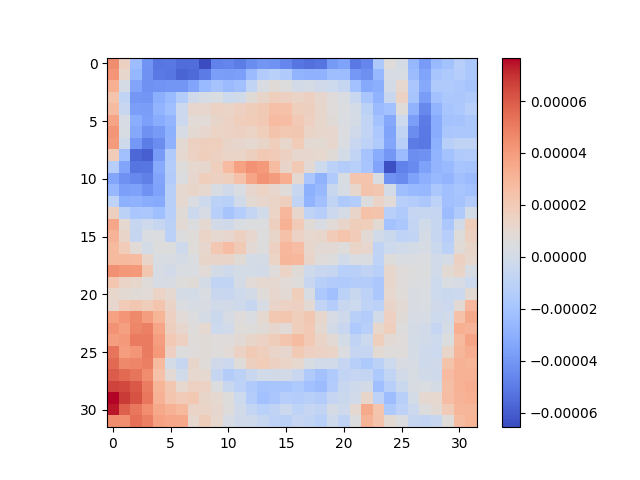
\includegraphics[width=40mm]{figure_2.png}
\end{figure}

The left figure is from full training and the right figure is from two image per person.

\section{Part 5}
The performance is below:
\newline 100 iamges for each person:
\\Training set: 299 and 300, 99.8\%
\\Validation set: 28 and 27, 91.7\%
\\act\_test: 238 and 263, 83.5\%
\\
\newline 75 iamges for each person: 
\\Training set: 225 and 225, 100\%
\\Validation set: 28 and 27, 91.7\%
\\act\_test: 228 and 267, 82.5\%
\\
\newline 50 iamges for each person: 
\\Training set: 150 and 150, 100\%
\\Validation set: 28 and 24, 86.7\%
\\act\_test: 232 and 241, 78.9\%
\\
\newline 25 iamges for each person: 
\\Training set: 75 and 75, 100\%
\\Validation set: 29 and 26, 91.7\%
\\act\_test: 236 and 219, 75.8\%
\\

\begin{tikzpicture}
\begin{axis}[
    title={Training set performance},
    xlabel={size},
    ylabel={performance},
    xmin=0, xmax=100,
    ymin=0, ymax=100,
    xtick={0,25,50,75,100},
    ytick={0,25,50,75,100},
    grid style=dashed,
]
 
\addplot[
    color=blue,
    mark=square,
    ]
    coordinates {
    (25,100)(50,100)(75,100)(100,99.8)
    };
\end{axis}
\end{tikzpicture}

\begin{tikzpicture}
\begin{axis}[
    title={Validation set performance},
    xlabel={size},
    ylabel={performance},
    xmin=0, xmax=100,
    ymin=0, ymax=100,
    xtick={0,25,50,75,100},
    ytick={0,25,50,75,100},
    grid style=dashed,
]
 
\addplot[
    color=blue,
    mark=square,
    ]
    coordinates {
    (25,91.7)(50,86.7)(75,91.7)(100,91.7)
    };
\end{axis}
\end{tikzpicture}

\begin{tikzpicture}
\begin{axis}[
    title={act\_test set performance},
    xlabel={size},
    ylabel={performance},
    xmin=0, xmax=100,
    ymin=0, ymax=100,
    xtick={0,25,50,75,100},
    ytick={0,25,50,75,100},
    grid style=dashed,
]
 
\addplot[
    color=blue,
    mark=square,
    ]
    coordinates {
    (25,75.8)(50,78.9)(75,82.5)(100,83.5)
    };
\end{axis}
\end{tikzpicture}

\clearpage
\section{Part 6}
\subsection{a)}
\begin{figure}[ht!]
  \includegraphics[width=170mm]{6a.jpg}
\end{figure}

\clearpage
\subsection{b)}
$$\frac{\partial J(\theta)}{\partial \theta}$$
\\
$$=\frac{\partial (\theta^TX-Y)^T(\theta^TX-Y)}{\partial \theta}$$
\\
$$=\frac{\partial (X^T\theta\theta^TX-Y^T\theta^TX-X^T\thetaY+Y^TY)^T(\theta^TX-Y)}{\partial \theta}$$
\\
$$=\frac{\partial (X^T\theta\theta^TX-2Y^T\theta^TX+Y^TY}{\partial \theta}$$
\\
$$=\frac{\partial (X^T(\theta)^2X-2Y^T\theta^TX+Y^TY}{\partial \theta}$$
\\
$$=2XX^T\theta-2XY^T$$
\\
$$=2X(X^T\theta-Y^T)$$
\\
$$=2X(\theta^TX-Y)^T$$

\subsection{c)} The code for my newf and newdf:
\begin{lstlisting}
def newf(x,y,theta):
    return sum((dot(theta.T,x)-y)**2)

def newdf(x,y,theta):
    return (dot(x.T,(dot(x,theta)-y))*2)
\end{lstlisting}

\subsection{d)}
In this part, I check for three pairs of data.
\\First, I check 1st row and 2nd column:
\\Limit: -3.56727620776
\\Gradient descent: -3.56727618536
\\First, I check 1st row and 1st column:
\\Limit: -1.58994404309
\\Gradient descent: -1.5894405675
\\First, I check 0th row and 2nd column:
\\Limit: -3.32390110991
\\Gradient descent: -3.32390111448
\\From above we find that the results are almost the same using two different method.
\\The code to achieve this is below:
\begin{lstlisting}
def limit(x,y,theta,a,b):
    h=1e-8
    list_h=[[0,0,0],[0,0,0],[0,0,0]]
    list_h[a][b]=h
    return (newf(x,y,theta+array(list_h))-newf(x,y,theta-array(list_h)))/(2*h)
    
def part6d(a,b):
    test_x=array(([3,2,1],[2,1,2],[0,1,1],[2,1,0]))
    test_y=array(([1,0,0],[0,1,0],[1,0,1],[0,0,1]))
    init_theta=array([[0.]*3]*3)
    theta=grad_descent(newf,newdf,test_x,test_y,init_theta,1e-7)
    print "using limit"
    print limit(test_x,test_y,theta,a,b)
    print "using gradient descent"
    print newdf(test_x,test_y,theta)[a][b]
\end{lstlisting}

\section{Part 7}
After I run gradient descent on the set of six actors act in order to perform face recognition, I got performance below:
\\Training set performance: [91, 93, 94, 96, 85, 88], 91.2\%
\\Validation set performance: [10, 6, 10, 9, 8, 10], 88.3\%
\\
\\For gradient descent, I choose parameter f, df, x, y, init\_t, and $\alpha$. These parameter make sense because we have to use them: f is the cost function, df is derivative $df/d\theta$, x contains all the training data, y contains all the labels of images, and $\alpha$ is used to move $\theta$ properly.

\clearpage
\section{Part 8}
\begin{figure}[ht!]
  \includegraphics[width=60mm]{baldwin.png} \hfill
  \includegraphics[width=60mm]{carell.png}
  \newline Baldwin\ \ \ \ \ \ \ \ \ \ \ \ \ \ \ \ \ \ \ \ \ \ \ \ \ \ \ \ \ \ \ \ \ \ \ \ \ \ \ \ \ \ \ Carell
\end{figure}\

\begin{figure}[ht!]
  \includegraphics[width=60mm]{chenometh.png} \hfill
  \includegraphics[width=60mm]{descher.png}
  \newline Chenoweth\ \ \ \ \ \ \ \ \ \ \ \ \ \ \ \ \ \ \ \ \ \ \ \ \ \ \ \ \ \ \ \ \ \ \ \ \ \ \ \ \ \ \ Descher
\end{figure}

\begin{figure}[ht!]
  \includegraphics[width=60mm]{ferrera.png} \hfill
  \includegraphics[width=60mm]{hader.png}
  \newline Ferrera\ \ \ \ \ \ \ \ \ \ \ \ \ \ \ \ \ \ \ \ \ \ \ \ \ \ \ \ \ \ \ \ \ \ \ \ \ \ \ \ \ \ \ Hader
\end{figure}

\end{document}